
\documentclass[xcolor=dvipsnames, mathserif, 10pt]{beamer}


\setbeamercolor{normal text}{fg=black,bg=white}

%\setbeamercolor{alerted text}{bg=white,fg=brown}



\mode<presentation>
{
  \usetheme{Frankfurt}
   \setbeamercovered{transparent}
}

\usepackage{cancel}
\newcommand{\argmin}{\operatorname{argmin}}
\usepackage{adjustbox}
%\definecolor{mygreen}{cmyk}{0.82,0.11,1,0.25}
\setbeamertemplate{blocks}[rounded][shadow=false]
\addtobeamertemplate{block begin}{\pgfsetfillopacity{0.8}}{\pgfsetfillopacity{1}}
\setbeamercolor{structure}{fg=Sepia}
\setbeamercolor*{block title example}{fg=white,
bg= OliveGreen}
\setbeamercolor*{block body example}{fg= black,
bg= Green!5}

\usepackage{etex}
\usepackage[utf8]{inputenc}
\usepackage[english]{babel}
\usepackage{amsmath,amsfonts,amsthm,float,graphicx,graphics,tabularx}
\usepackage{dcolumn}
\usepackage{algpseudocode}
\usepackage{lmodern}
\usepackage{morefloats}
\usepackage{alltt,booktabs,epstopdf}
\usepackage[ruled,vlined,linesnumbered]{algorithm2e}
\usepackage[nocomma]{optidef}
\usepackage{float}
\usepackage{bigstrut}
\usepackage{multirow}
\usepackage[style=verbose,backend=biber]{biblatex}
\addbibresource{biblist.bib}
\newcommand{\T}{\mathcal{T}}

\DeclarePairedDelimiter\ceil{\lceil}{\rceil}
\DeclarePairedDelimiter\floor{\lfloor}{\rfloor}
\setbeamertemplate{footline}[frame number]

\setbeamercolor{alerted text}{fg=Sepia}
\setbeamertemplate{items}[square]
\setbeamertemplate{navigation symbols}{}
\newcommand{\bmin}{\underline{b}}
\newcommand{\Prob}{\mathbb{P}}
\usepackage{tikz}
\usetikzlibrary{shapes.geometric, arrows}

\usepackage{amsmath,amsfonts,amsthm,float,graphicx,graphics}
\usepackage{dcolumn}
\usepackage{algpseudocode}
\usepackage{lmodern}
\usepackage{morefloats}
\usepackage{alltt,booktabs,epstopdf}
\usepackage{subfigure}
\usepackage[justification=centering]{caption}
\usepackage{lipsum}
\usepackage{graphicx}
\usepackage{caption}
\newcommand{\X}{\mathcal{X}}
\newcommand{\hoff}{\mathcal{H}_{A,b}}
\newcommand{\hoffp}{\overline{\mathcal{H}}_{A}}



\newcommand{\eps}{\epsilon}
 \newcommand\R{{\sf I\kern-0.1em R}}
 \newcommand{\tr}{^\intercal}
 \newcommand{\st}{\mbox{ \rm s.t.}}
 \newcommand\one{{\sf 1\kern-0.37em 1}}
 \newcommand{\refer}[1]{\mbox{\rm(\ref{#1})}}
 \newcommand{\dsum}{\displaystyle\sum}

\algrenewcommand\algorithmicindent{0.5em}%
\newcommand{\B}{\mathcal{B}}
\newcommand{\I}{\mathcal{I}}
\newcommand{\J}{\mathcal{J}}
\renewcommand{\L}{\mathcal{L}}
\newcommand{\Exp}{\mathbb{E}}

\newcommand{\bx}{\hbox{$x\! \circ \! x$}}
\newcommand{\brac}[1]{\left( #1 \right)}
\newcommand{\ip}[2]{\langle #1 , #2 \rangle}    % inner product
\newcommand{\hd}{{\widehat d}}
\newcommand{\QM}{\mathcal{M}}
\renewcommand{\P}{\mathcal{P}}

%\newcommand{\hilight}[1]{\colorbox{LightBlue}{#1}}
%\newcommand{\hilight}[1]{\colorbox{LightYellow}{#1}}
\newcommand{\matr}[1]{\begin{bmatrix} #1 \end{bmatrix}}    % matrix

%\newcommand{\frametitle}[1]{{\large\bf\color{blue} #1}}



\newcommand\N{\mathbb N}
%\newcommand\R{\mathbb R}
\renewcommand\S{\mathbb S}
\newcommand{\ns}[1]{\overline{#1}} % "non-standard" extension -- may
\newcommand{\copos}{\operatorname{Copos}}

%\newcommand\R{{\bf R}}
%\renewcommand\S{{\bf S}}
\newcommand{\pf}{\noindent{\em Proof. }}
%\newcommand{\st}{\mbox{ \rm s.t. }}
%\newcommand{\st}{\operatorname{s.t.\text{ }}}
%\newcommand{\st}{\operatorname{s.t.}}
%\newcommand{\qed}{\hfill \mbox{$\Box$}}
\newcommand{\distSing}[1]{\mbox{\rm dist}(#1,\mbox{\rm Sing})}
\newcommand{\reldistSing}[1]{\mbox{\rm reldist}(#1,\mbox{\rm Sing})}
\newcommand{\distInf}[1]{\mbox{\rm dist}(#1,\mathcal I)}
\newcommand{\distSSing}[1]{\mbox{\rm dist}_E(#1,\mbox{\rm Sing})}
\newcommand{\distSpar}[1]{\mbox{\rm dist}_E(#1,\mathcal I)}
\newcommand{\blockdist}[1]{\mbox{\rm dist}_{\bf \Delta}(#1,\mathcal I)}
\newcommand{\blockalphadist}[1]{\mbox{\rm dist}_{\bfD,\alpha}(#1,\mathcal I)}
\newcommand{\reldist}[1]{\mbox{\rm dist}(#1,\mathcal I)}
\newcommand{\dom}{\mbox{\rm dom}}
\newcommand{\reg}{\mbox{\rm reg}}
%\newcommand{\refer}[1]{\mbox{\rm(\ref{#1})}}
\newcommand{\smfrac}[2]{ \frac{#1}{#2} }
\newcommand{\x}{\times}
%\newcommand{\X}{\mbox{\rm X}}
\newcommand{\Xomit}[1]{}
\newcommand{\rpi}{{\color{blue} \pi}}
%\newcommand{\res}[1]\alert{{#1}}
\newcommand{\cvar}{\mbox{ \rm CVaR}}
\newcommand{\wcvar}{\mbox{ \rm WCVaR}}
\newcommand{\conv}{\operatorname{conv}}

\newcommand{\dmin}{\displaystyle\min}
\newcommand{\closure}{\operatorname{cl}}
\newcommand{\supe}{\sup\text{ }}

\newcommand{\sgn}{\mbox{\rm sgn}}

\newcommand\A{\mathcal A}
%\newcommand\B{\mathbb B}
%\newcommand\R{\mathbb R}
%\newcommand\R{{\sf I\kern-0.1em R}}
\newcommand{\blue}[1]{{\color{blue} #1}}
\newcommand{\convex}{\operatorname{conv}}
\newcommand{\cone}{\operatorname{cone}}
\newcommand{\mat}[2]{{\left[\begin{array}{#1}#2\end{array}\right]}}
\newcommand{\sos}{{\rm sos}}


%\newcommand\I{\mathcal I}
\newcommand\bfD{{\bf \Delta}}
%\newcommand{\ones}{ee\transp}
\newcommand\ones{\hbox{1\hspace{-3pt}I}}
\newcommand\K{\mathcal K}
\newcommand\Q{\mathcal Q}
\newcommand\C{\mathcal C}
\newcommand\E{\mathcal E}
%\newcommand{\tr}{{\rm \tiny T}}



\newtheorem{prop}{Proposition}
\newtheorem{thm}{Theorem}
\newtheorem{corol}{Corollary}
\newtheorem{conj}{Conjecture}
%\newtheorem{lemma}[prop]{Lemma}
\newtheorem{remark}[prop]{Remark}
\newtheorem{proposition}[prop]{Proposition}
\newtheorem{claim}[prop]{Claim}
\def\vx{\vec{\kern1pt x}}
\def\vy{\vec{\kern1pt y}}
\def\vs{\vec{\kern1pt s}}
\def\vw{\vec{\kern1pt w}}
\renewcommand\b{\vec{\kern1pt b}}
\renewcommand\c{\vec{\kern1pt c}}
\newcommand{\nhd}[1]{#1^\perp}

\newcommand{\rec}[1]{{#1}^\infty}


\tikzstyle{customer} = [rectangle, minimum width=2cm, minimum height=0.7cm,text centered, draw=black, fill=red!30]



\tikzstyle{plant} = [rectangle, minimum width=2cm, minimum height=0.7cm, text centered, draw=black, fill=orange!30]



\tikzstyle{meter} = [circle, text centered, draw=black, fill=green!30, inner sep=0cm,minimum size=0.2cm]

\tikzstyle{arrow} = [thick,->,>=stealth]


\setbeamercovered{invisible}



\title[]
{A Branch-and-Price Algorithm for Combined Location and Routing Problems Under Capacity Restrictions}


\author[\textbf{Samira Fallah} \and Lawrence V. Snyder \and Theodore K. Ralphs]{%
  \texorpdfstring{%
  \vspace{10pt}
    \begin{columns}
      \column{.25\linewidth}
      \centering
      \textbf{\small Samira Fallah} \\ \texttt{\small saf418@lehigh.edu}
      \column{.25\linewidth}
      \centering
      {\small Lawrence V. Snyder} \\ \texttt{\small lvs2@lehigh.edu}
      \column{.25\linewidth}
      \centering
      {\small Theodore K. Ralphs} \\ \texttt{\small ted@lehigh.edu}
    \end{columns}
    \vspace{5pt}
 }
 {Author 1, Author 2, Author 3}
}

\institute{\\ \vspace{10pt} 
\includegraphics[height=3cm,width=9cm]{LehighLogo.png}}
\date[]
{\\
October 29, 2020}


% ToC command
\AtBeginSubsection[]
{
  \begin{frame}<beamer>{Outline}
    \tableofcontents[currentsection,currentsubsection]
  \end{frame}
}



\logo{
\includegraphics[height=0.5cm]{logo}}
%\logo{\tdtime}
\newcommand{\excl}[1]{\section{exclude}}

\makeatletter
\def\sectionentry#1#2#3#4#5{% section number, section title, page
  \beamer@xpos=0\relax%
  \beamer@ypos=1\relax%
  \beamer@ypos@offset=0\relax%
  \ifnum#5=\c@part%
  \beamer@section@set@min@width%
  \box\beamer@sectionbox\hskip1.875ex plus 1fill%
  \setbox\beamer@sectionbox=
  \hbox{\def\insertsectionhead{#2}%
    \def\insertsectionheadnumber{#1}%
    \def\insertpartheadnumber{#5}%
    {%
      \usebeamerfont{section in head/foot}\usebeamercolor[fg]{section in head/foot}%
      \ifnum\c@section=#1%
        \hyperlink{Navigation#3}{{\usebeamertemplate{section in head/foot}}}%
        :~\insertsubsectionhead%
      \else%
        \hyperlink{Navigation#3}{{\usebeamertemplate{section in head/foot shaded}}}%
      \fi}%
  }%
  \ht\beamer@sectionbox=1.875ex%
  \dp\beamer@sectionbox=0.75ex%
  \fi\ignorespaces} 
\makeatother

\begin{document}

\begin{frame}[plain]
    \titlepage
\end{frame}

\begin{frame}
\frametitle{Outline}
  \tableofcontents
\end{frame}


\section{Introduction}
\begin{frame}{Introduction}
Motivation: where to locate the facilities and how to allocate customers to the selected facilities with capacity constraints on both the facilities and the vehicles to minimize the total cost.



\end{frame}

\begin{frame}{Literature}
\begin{itemize}
    \item Heuristics
    \begin{itemize}
        \item Construction and Improvement
        \item Clustering Algorithms
        \item Metaheuristics
    \end{itemize}
    \item Optimization-Based Approaches
    \begin{itemize}
        \item Benders' Decomposition
        \item Dynamic Programming
        \item Polyhedral Approach
        \item Matching-Based Approach
        \item Column Generation
    \end{itemize}
\end{itemize}
   
\end{frame}
\section{Problem Definition}
\begin{frame}{Problem Definition and Formulations}
Objective: to determine the number and location of facilities and construct a set of vehicle routes from facilities to customers to
minimize total cost.
\vskip 3
Total cost: both the fixed and operating costs of  facilities and vehicles.
\vskip 3
Two Types of formulation:
\begin{itemize}
    \item Vehicle Flow Formulation
    \item Set-Partitioning Formulation
\end{itemize}
\end{frame}

\begin{frame}{Vehicle Flow Formulation \footcite{akca2009branch}}
Notations:

$I:$ the set of customers,
\vskip 3
$J:$ the set of candidate facilities,
\vskip 3
$V = I \cup J$,
\vskip 3

Extra assumption: assume that each facility has its own set of vehicles,
\vskip 3
$H_j:$ the set of vehicles located at facility $j$, $\forall j \in J$,
\vskip 3
$H$: the set of all vehicles,
\vskip 3

\end{frame}


\begin{frame}{Vehicle Flow Formulation-Cont}
\begin{figure}[H]
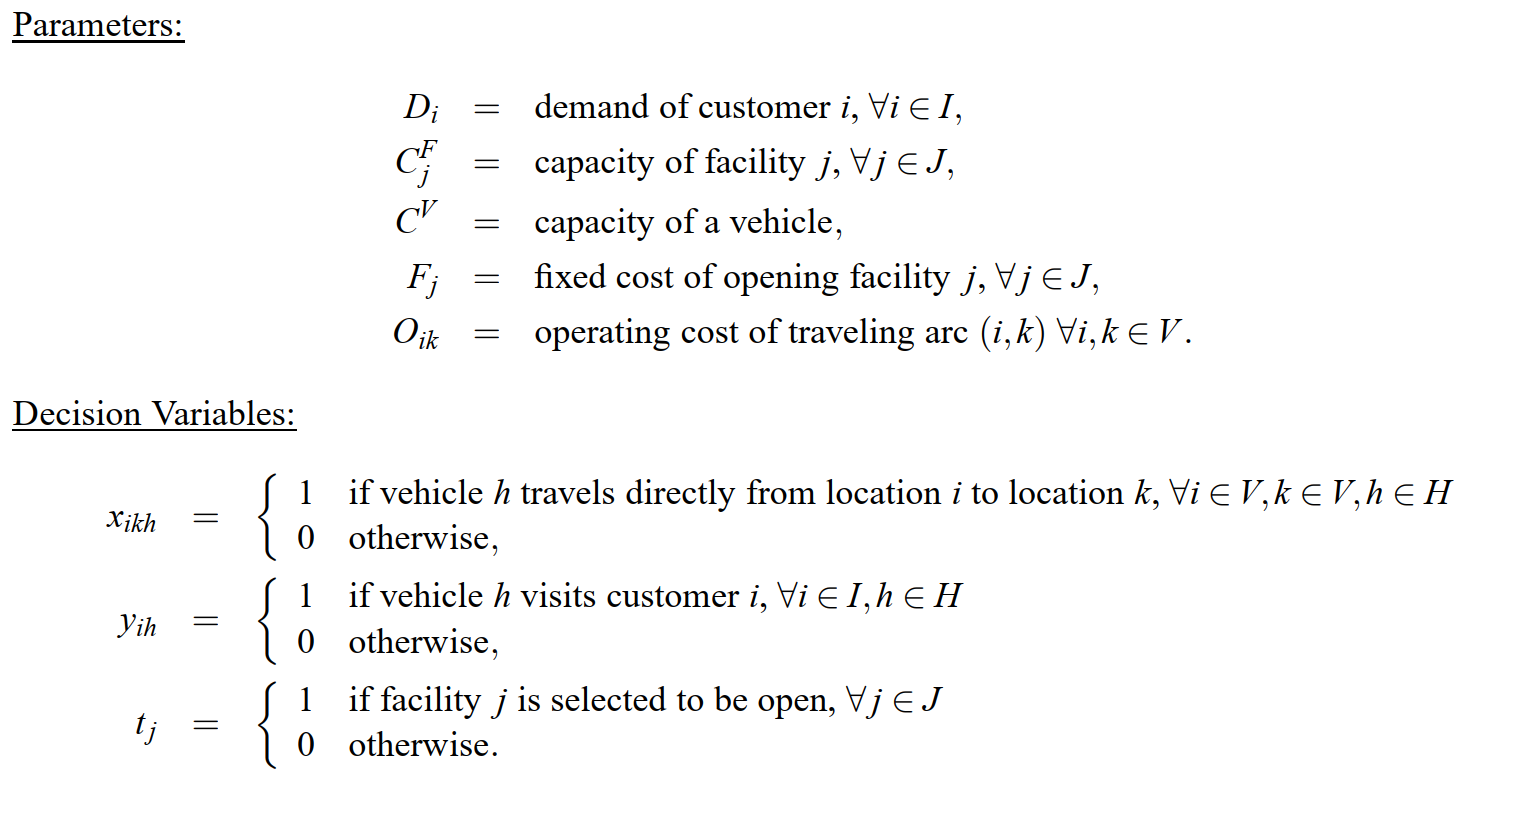
\includegraphics[width=11cm]{Flow.PNG}
\end{figure} 
\end{frame}


\begin{frame}{Vehicle Flow Formulation-Cont}
\begin{figure}[H]
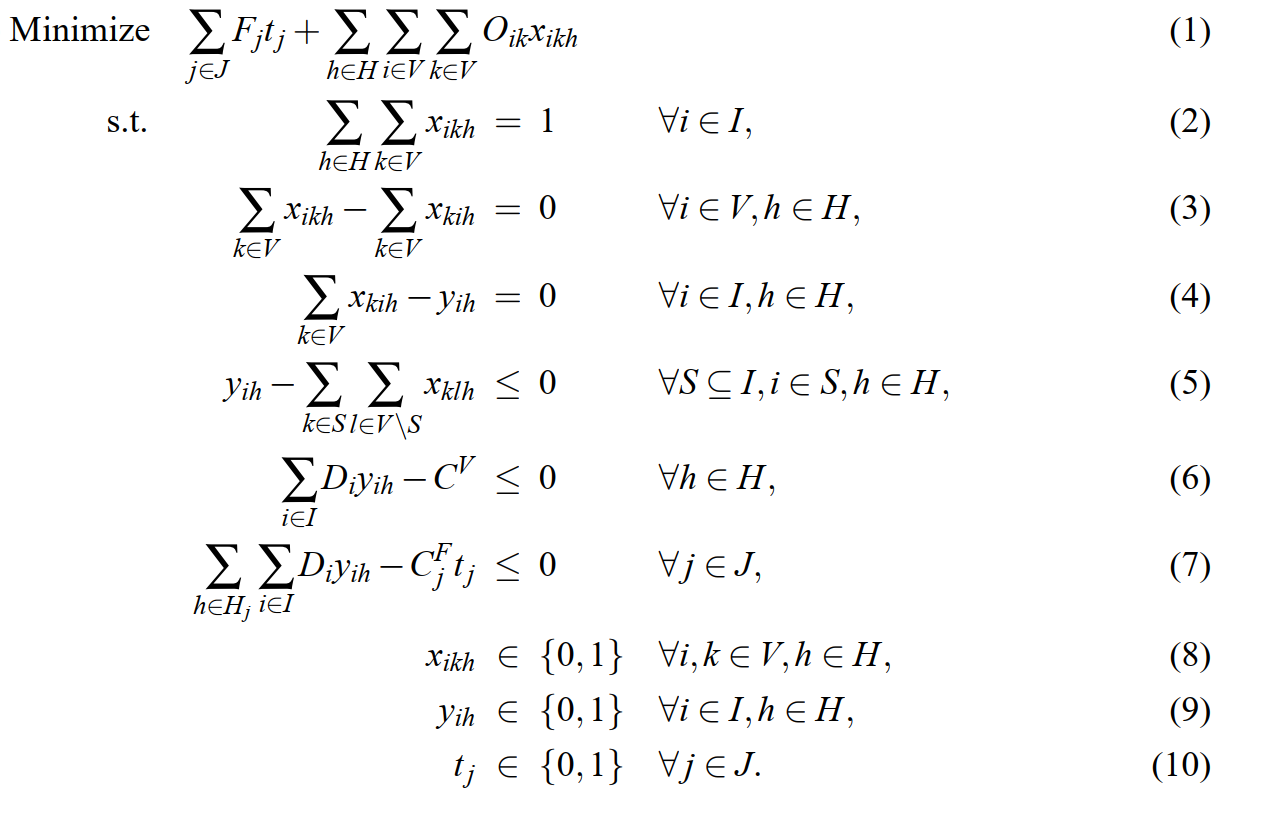
\includegraphics[width=10cm]{FlowFormulation.PNG}
\end{figure} 
\end{frame}



\section{Solution Methods}
\begin{frame}{Branch and Price Framework}
\begin{itemize}
    \item The number of routes will be too large!
    \item To solve the LP relaxation of models with exponentially many columns, column generation algorithms can be used.
    \item By adding eligible columns dynamically to enter the basis, we generate only those columns that may improve the objective function.
    \vskip 6mm
    \item We used DipPy from COIN-OR\footcite{coinor} organization as the framework.
    \item DipPy itself reformulate our problem to the set-partitioning formulation.
    \begin{itemize}
    \item The Restricted Master Problem (RMP) is the set-partitioning formulation with a subset of routes.
        \item The subproblem is to find a route for a specific vehicle that can improve the objective of the RMP.
    \end{itemize}
    
\end{itemize}

\end{frame}

\begin{frame}{Branch and Price Framework\footcite{branchandprice}}
\begin{figure}[H]
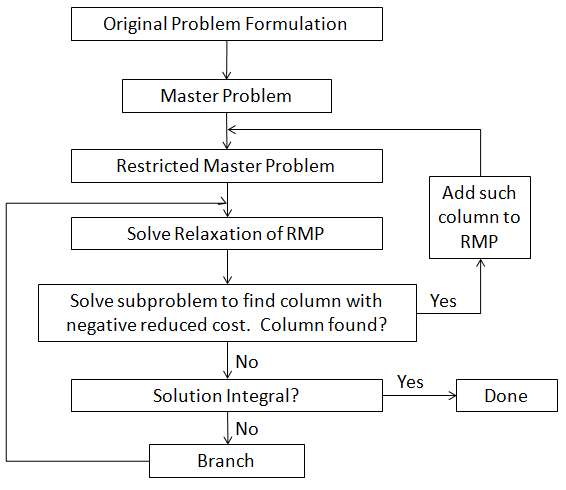
\includegraphics[width=8cm]{Branch_and_price_diagram.png}
\end{figure}  


\end{frame}

\begin{frame}{Branch and Price Framework}
\begin{figure}[H]
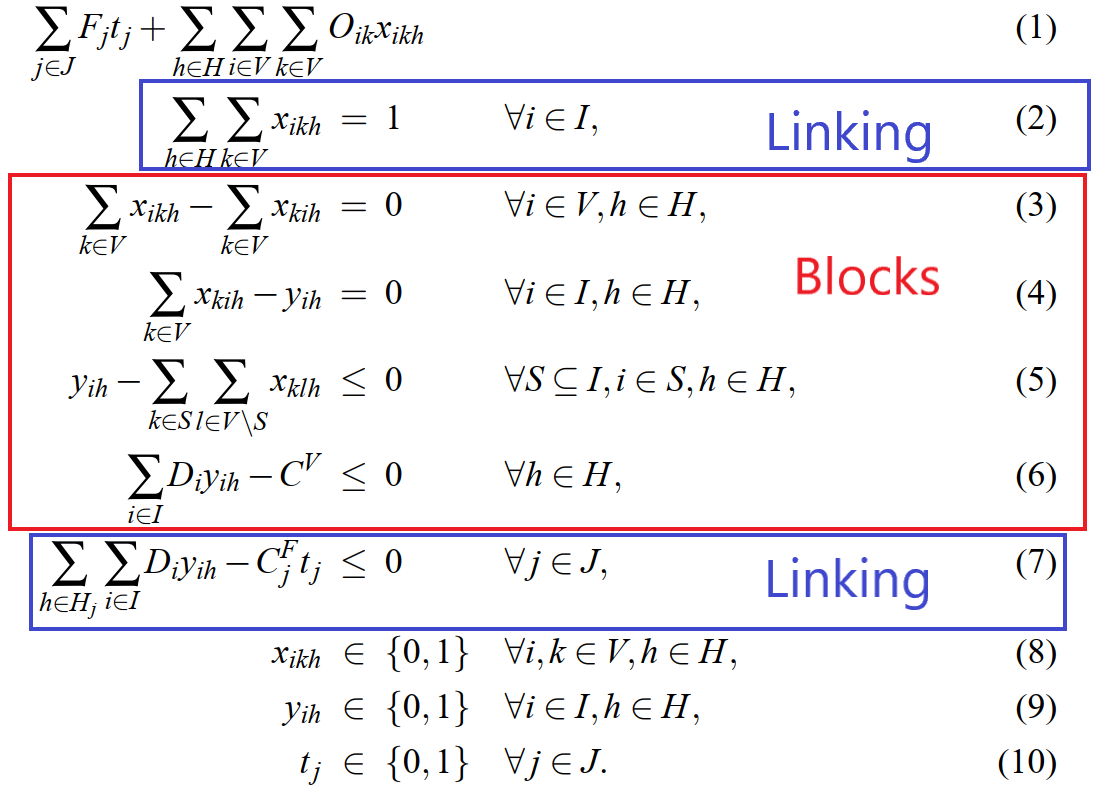
\includegraphics[width=8cm]{FlowFormulationEdited.png}
\end{figure}  

\end{frame}

\begin{frame}{Some Modifications}
I ignored the subtour elimination constraints since I solved my subproblem with dynamic programming.
\vskip 3mm
In addition, I added two other constraints:
\begin{itemize}
    \item These constraints prevent assigning the vehicles that are specified for the specific facility to the route originating from other facilities:
    
    $$X_{jkh}=0 \quad j \in J, k \in I, h \in (H \setminus H_j),$$
    
    \item and these constraints prevent self cycling:
    $$X_{iih}=0 \quad i \in V, h \in H.$$
\end{itemize}


\end{frame}

\begin{frame}{Solve Subproblem-Exact}
Our subproblem: the Elementary Shortest Path Problem with Resource Constraints (ESPPRC).
\vskip 3
We used Feillet's Label Setting algorithm \footcite{feillet2004exact} for solving ESPPRC.
\vskip 3
Some basics of Feillet's Algorithm:
\vskip 3
A node is unreachable:
\begin{itemize}
    \item If they have already been visited in the path, or
    \item If they cannot be served by the vehicle without violating a resource constraint.
\end{itemize}
\end{frame}


\begin{frame}{Solve Subproblem-Exact-Cont.}

For each node we have list of labels like
$\{L_1^i, L_2^i, \hdots, L_\mu^i\}$ in which there are information about one path of node $i$.
\vskip 3
$L_1^i = <R_C^i, R_V^i, R_n^i, V_1^i,\hdots,V_I^i>$
\vskip 3
$R_C^i = \text{Total cost so far}$,
\vskip 3
$R_V^i = \text{Total demands so far}$,
\vskip 3
$R_n^i = \text{Total number of unreachable nodes}$,
\vskip 3
$V_k^i$: status of going from $i$ to $k$,
\vskip 3
\begin{equation*}
  V_k^i=\begin{cases}
    -1, & \text{if node $k$ is unreachable due to capacity constraint},\\
    0, & \text{if node $k$ is reachable and is not in the path so far},\\
    s>0, & \text{if node $k$ is the s'th node in the path.}
  \end{cases}
\end{equation*}

\end{frame}


\begin{frame}{Solve Subproblem-Exact-Cont.}
\begin{itemize}
    \item Initialization Step:
    \begin{itemize}
        \item Label list is created for each node to keep the generated labels.
        \item All label lists (except the list for the source node) are initially empty.
        \item The source has one label, which is a zero vector.
    \end{itemize}
   
\end{itemize}

\end{frame}

\begin{frame}{Solve Subproblem-Exact-Cont.}
\begin{itemize}
    

 \item Extension step
    \begin{itemize}
        \item For each node, all unprocessed labels are extended to all possible successors. The label $l_r^i$ for node $i$ can be extended to node $k$ if
\begin{itemize}
    \item node k is reachable, i.e., $V^i_k=0$, 
    \item the path is feasible, i.e., $R_k_v+D_g \leq C^k$.
\end{itemize}
        

\item If it is feasible to extend $l_r^i$ to node $k$, a new label is created for node $k$ by updating the resource consumptions as follows:
\begin{itemize}
    \item  $R_c_k = R_c^i + C_{ik}$
    
    \item $R_v_k = R_v^i + D_{k}$
    
    \item We update the status of nodes on the labels as follows:
    \begin{equation*}
  V_g^k=\begin{cases}
    V_g^i, & \text{if $V_g^i \neq 0$},\\
    0, & \text{if $V_g^i = 0$ and $R_v^k + D_g > C^k$},\\
    N, & \text{if $g=k$ and $N$ is the $\#$ of nodes in path},\\
    0, & \text{o/w}.
  \end{cases}
\end{equation*}
  \end{itemize}  
\end{itemize}

\end{itemize}
\end{frame}

\begin{frame}{Solve Subproblem-Exact-Cont.}
\begin{itemize}
    \item Elimination step: After extension step we apply dominance properties rule to the newly generated labels. Label 1 dominates label 2, if:
    \begin{itemize}
        \item $(R_v^k)^1 \leq (R_v^k)^2$,
        \item $(R_C^k)^1 \leq (R_C^k)^2$,
        \item if node $g$ is unreachable in 1, it is unreachable in 2. 
    \end{itemize}
\end{itemize}
\end{frame}


\begin{frame}{Solve Subproblem-Heuristics.}
\begin{itemize}
    
    \item Heuristic\_CS:
    We set the limit to the size of the customers considered in each pricing problem with \textit{minimum spanning tree} algorithm.
    
    \item Heuristic\_LL: We set the limit on the size of the labels in each node.
    
\end{itemize}
\end{frame}

\begin{frame}{Computational Experiments}

% Table generated by Excel2LaTeX from sheet 'Sheet3'
\begin{table}[htbp]
  \centering
  %\caption{Add caption}
  \adjustbox{max height=\dimexpr\textheight-5.75cm\relax,
           max width=\textwidth}{
   \begin{tabular}{|c|c|c|c|c|c|c|c|c|c|}
\cline{2-10}    \multicolumn{1}{c|}{} & \textit{B\&P} & \multicolumn{2}{c|}{\textit{Heur\_CS5}} & \multicolumn{2}{c|}{\textit{Heur\_CS10}} & \multicolumn{2}{c|}{\textit{Heur\_LL5}} & \multicolumn{2}{c|}{\textit{Heur\_LL10}} \bigstrut\\
    \hline
    \multirow{2}[2]{*}{\textit{ID}} & \multicolumn{1}{p{3.065em}|}{\textit{Time}} & \multicolumn{1}{p{2.565em}|}{\textit{Time}} & \multicolumn{1}{p{2em}|}{\textit{Opt.}} & \multicolumn{1}{p{2.565em}|}{\textit{Time}} & \multicolumn{1}{p{2.135em}|}{\textit{Opt.}} & \multicolumn{1}{p{2.235em}|}{\textit{Time}} & \multicolumn{1}{p{2.135em}|}{\textit{Opt.}} & \multicolumn{1}{p{2.565em}|}{\textit{Time}} & \multicolumn{1}{p{2.135em}|}{\textit{Opt.}} \bigstrut[t]\\
          & \multicolumn{1}{p{3.065em}|}{\textit{(sec)}} & \multicolumn{1}{p{2.565em}|}{\textit{(sec)}} & \multicolumn{1}{p{2em}|}{\textit{Gap}} & \multicolumn{1}{p{2.565em}|}{\textit{(sec)}} & \multicolumn{1}{p{2.135em}|}{\textit{Gap}} & \multicolumn{1}{p{2.235em}|}{\textit{(sec)}} & \multicolumn{1}{p{2.135em}|}{\textit{Gap}} & \multicolumn{1}{p{2.565em}|}{\textit{(sec)}} & \multicolumn{1}{p{2.135em}|}{\textit{Gap}} \bigstrut[b]\\
    \hline
    \textit{r15x6\_a\_1} & \textbf{857} & \textbf{1581} & \textbf{0.00} & \textbf{933} & \textbf{0.00} & \textbf{1601} & \textbf{0.00} & \textbf{778} & \textbf{0.00} \bigstrut\\
    \hline
    \textit{r15x6\_a\_2} & \textbf{732} & 530   & 0.02  & \textbf{558} & \textbf{0.00} & 630   & 0.02  & \textbf{541} & \textbf{0.00} \bigstrut\\
    \hline
    \textit{r15x6\_a\_3} & \textbf{1167} & \textbf{759} & \textbf{0.00} & \textbf{885} & \textbf{0.00} & \textbf{736} & \textbf{0.00} & \textbf{935} & \textbf{0.00} \bigstrut\\
    \hline
    \textit{r15x6\_a\_4} & \textbf{1042} & \textbf{731} & \textbf{0.00} & \textbf{611} & \textbf{0.00} & \textbf{627} & \textbf{0.00} & \textbf{600} & \textbf{0.00} \bigstrut\\
    \hline
    \textit{r15x6\_a\_5} & \textbf{691} & \textbf{558} & \textbf{0.00} & \textbf{684} & \textbf{0.00} & \textbf{563} & \textbf{0.00} & \textbf{673} & \textbf{0.00} \bigstrut\\
    \hline
    \textit{r15x6\_a\_6} & \textbf{14891} & \textbf{665} & \textbf{0.00} & \textbf{2250} & \textbf{0.00} & \textbf{658} & \textbf{0.00} & \textbf{2231} & \textbf{0.00} \bigstrut\\
    \hline
    \textit{r15x6\_a\_7} & \textbf{84933} & 4402  & 0.06  & \textbf{17494} & \textbf{0.00} & 5870  & 0.07  & \textbf{17489} & \textbf{0.00} \bigstrut\\
    \hline
    \textit{r15x6\_a\_8} & \textbf{7099} & 11317 & 0.08  & \textbf{1508} & \textbf{0.00} & 1908  & 0.10  & \textbf{1483} & \textbf{0.00} \bigstrut\\
    \hline
    \textit{r15x6\_b\_3} & \textbf{210084} & \textbf{1056} & \textbf{0.00} & \textbf{17508} & \textbf{0.00} & \textbf{918} & \textbf{0.00} & \textbf{17484} & \textbf{0.00} \bigstrut\\
    \hline
    \textit{r20x8\_a\_2} & \textbf{9121} & 7085  & 0.02  & 8195  & 0.01  & 5741  & 0.02  & 7275  & 0.01 \bigstrut\\
    \hline
    \textit{r20x8\_a\_3} & \textbf{8433} & 7029  & 0.08  & \textbf{7254} & \textbf{0.00} & 7263  & 0.08  & \textbf{6216} & \textbf{0.00} \bigstrut\\
    \hline

    \end{tabular}}
  \label{tab:addlabel}%
\end{table}%
$$C^V= (1-\alpha)\max_{i \in I}({D_i})+ \alpha(\sum_{i \in I} D_i)$$
$$\alpha=\{0, 0.25, 0.5, 0.75, 1\}$$

\end{frame}

\begin{frame}{Some Observations}
\begin{itemize}
    \item Heuristic method CS5: 
    \begin{itemize}
        \item Average optimality gap of the solution is 5\%,
        \item About 50.6\% reduction in execution time.
    \end{itemize} 
    \vskip 5
    \item Heuristic method CS10: 
    \begin{itemize}
        \item Average optimality gap of the solution is 0.1\%,
        \item About 40\% reduction in execution time.
    \end{itemize}
      \vskip 5
    \item Heuristic method LL5:
    \begin{itemize}
        \item Average optimality gap of the solution is 3.2\%,
        \item About 32.4\% reduction in execution time.
    \end{itemize} 
     \vskip 5
    \item Heuristic method LL10: 
    
    \begin{itemize}
        \item Average optimality gap of the solution is 0.02\%,
        \item About 9.1\% reduction in execution time.
    \end{itemize} 
\end{itemize}

\end{frame}



\section*{End of Presentation}
\begin{frame}[noframenumbering]{Questions?}
\centering \LARGE
  \emph{Thank you!}
\end{frame}




\end{document} 